\chapter{Balancing Unevenly Distributed Data in Seismic Tomography: {A} Global Adjoint Tomography Example\label{ch:weighting}}

\textbf{Note}\\
This chapter has been submitted as a paper entitled ``Balancing Unevenly Distributed Data in Seismic Tomography: {A} Global Adjoint Tomography Example'' by Ruan, Y., Lei, w., Modrak, R., \"{O}rsvuran, R., Bozda\u{g}, E., and Tromp, J.\ to the \textit{Geophysical Journal International}.


\section{summary}
The uneven distribution of earthquakes and stations in seismic tomography leads to slower convergence of nonlinear inversions and spatial bias in inversion results.
Including dense regional arrays, such as USArray or Hi-Net, in global tomography causes severe convergence and spatial bias problems, against which conventional preconditioning  schemes are ineffective.
To save computational cost and reduce model bias, we propose a new strategy based on a geographical weighting of sources and receivers.
We validate this strategy in
a 2D global waveform inversion test and show that the new weighting scheme leads to a nearly two-fold reduction in model error and much faster convergence relative to a conventionally-preconditioned inversion.
We implement this geographical weighting strategy for global adjoint tomography.
\section{summary}

%%%%%------------------------------------------
%
%   1, 
%
%%%%---------------------------------------------
\section{Introduction}
%Highlight points:

The deployment of new global and regional seismographic stations has made  more data available for seismic tomography than ever before.
The spatial distribution of these stations remains highly lopsided, however, with limited Ocean Bottom Seismometers (OBSs) or ocean island stations,
%it's ocean island basalt, so I think it's also ocean island station
and fewer stations in the southern hemisphere than in the northern hemisphere. 
This uneven station coverage, combined with the uneven distribution of earthquakes dictated by plate tectonics, poses major challenges for the inverse problem.   In global adjoint tomography in particular, the large number of paths from subduction zones, such as Fiji-Tonga, to dense arrays,  such as USArray,  causes highly oscillatory behavior in model updates, hindering convergence~\cite{bozdaug2016global}. 

Since the first global tomographic study by~\cite{Dziewonski77}, uneven data coverage has been an issue of concern. 
The problem with a cluster of earthquakes or a dense receiver array is that data residuals are correlated, and large portions of data are in some sense redundant.  %This redundant information is then amplified in the inversion by force of numbers.    
The correlation of data residuals is reflected in the data covariance matrix: 
its diagonal terms are the measurement error of each datum, and off-diagonal 
terms indicate coherence between the errors of two corresponding data.
Ideally, data errors are independent, in which case only diagonal terms
need to be considered, and off-diagonal terms can be safely ignored.  When measurements are strongly 
correlated, the off-diagonal terms become relevant.  

Although uneven data coverage is a well-known issue in seismic tomography,
there is limited literature on how it should be properly dealt with.
In an important global seismic tomography study by~\cite{Li1996}, uneven data coverage was addressed by weighting the diagonal terms of the data covariance matrix according to how significant 
their errors are correlated with the errors of the other data.
The weighting function 
in this study ($\omega = \omega_e\, \omega_n  \,\omega_r$) consists of data errors 
($\omega_e$ --- the rms amplitude of a wave packet), data redundancy within a wave packet ($\omega_n$ --- the inverse of the square root of number of data), and data redundancy 
amongst wave packets sampling similar ray paths 
($\omega_r$ --- a geometrical relationship between a given source-receiver 
pair to all other pairs).
The final term addresses data covariance through a path weighting strategy and has been employed in a few subsequent global tomography studies \cite{SchaefferLebedev13}.  
In this paper, we adopt a similar but more general approach to handle unevenly distributed measurements.  

The effects of uneven data coverage depend to some extent on the model parameterization and 
regularization in a given inversion.  \cite{Boschi1999} examined the effects of uneven data 
coverage with differently parameterized and regularized inversions. They parameterized their global 
model in terms of both blocks and spherical harmonics.
Sparse data coverage in the southern hemisphere
produced fictitious model features, especially in the spherical harmonic model.
Applying stronger 
regularization or damping, however, more or less resolved the issue.
In other words, to resolve bias in inversions caused by uneven data coverage, we need to sacrifice resolution in well-covered regions through stronger damping.
Their experiments justify to some extend the use of 
strong damping in some global inversions~\cite{Masters1996,Antolik2003}.      

Besides geographical weighting, 
other strategies have been developed in different contexts~\cite{grand1994, s362ani, ritsema2011s40rts, Moulik2016}.
For instance, the use of weights based on analyst-assessed data quality or weights for jointly inverting disparate data types (e.g., seismic and gravity measurements). 
These weighting choices are sometimes ad hoc and vary from one practitioner to another.
In this study, we focus on weighting with the goal of balancing uneven data coverage, without drawing many connections with other types of weighting.
Since full-waveform adjoint tomography is computationally expensive, it is important to address slow convergence due to unevenly distributed data.  
Here, we focus on a robust weighting strategy that can be applied to 
unevenly distributed earthquakes and stations to balance their contributions.

\section{Weighting strategy}
\label{sec:dataproc}

\subsection{Measurements and Misfit Function}

Seismic waves sample different parts of Earth's interior at different dominant frequencies, so it is natural to 
categorize seismic signals in terms of their type and band.
In global adjoint tomography~\cite{bozdaug2016global, Lei2018}, we currently consider three period 
bands: 17--40~s,  40--100~s, and 90--250~s. 
Typically, we select body waves in the 17--40~s band,
body waves in the 40--100~s band,
surface waves in the 40--100~s band,
and surface waves in the 90--250~s band.
Within each band, we consider three-component 
seismograms rotated into vertical, radial, and transverse directions 
of motion, so in total there are twelve data categories, as summarized in 
Table~\ref{table:categories}. 

\begin{table}
\caption{\small{Measurement categories in global adjoint tomography~\cite{bozdaug2016global, Lei2018}.
Seismic waves are categorized in terms of complementary 
period bands on three components of motion.}}
\begin{tabular}{|c|c|c|c|}
\hline

~         &  Vertical (Z) & Radial (R) &  Transverse (T) \\
\hline
17--40~s           &   P-SV body waves                        & P-SV body waves                       & SH body waves   \\
40--100~s         &   P-SV body waves                        & P-SV body waves                       & SH body waves \\
40--100~s         &   Rayleigh waves                           & Rayleigh waves                           & Love waves \\
90--250~s         &   Rayleigh waves                           & Rayleigh waves                           & Love waves \\
\hline
\end{tabular}\\
\label{table:categories}
\end{table}

Considering all these data categories, along with all the sources and receivers available for an inversion, we define an overall data misfit
\begin{equation}
\label{eq:misfit}
\Phi = \sum_{s=1}^{S} \omega_s \sum_{c=1}^{C} \omega_{c} \sum_{r=1}^{R_{sc}} \omega_{scr} \sum_{w=1}^{N_{scr}} \omega_{scrw}\, \chi_{scrw}
\quad .
\end{equation}
Here, $s = 1, ... , S$ denotes a given source and~$S$ the total number of sources.  Likewise, $c = 1, ..., C$ denotes a given category and~$C$  the total number of categories (in our case, the twelve categories summarized in Table~\ref{table:categories}).
$R_{sc}$ denotes the number of receivers for a given source~$s$ and category~$c$. Finally, $N_{scr}$ denotes the number of measurement windows for a given source~$s$, category~$c$, and receiver~$r$.

The misfit for a given source~$s$,
category~$c$, receiver~$r$, and measurement window~$w$ is
\begin{equation}
\label{eq:misfit_def}
\chi_{scrw} = \left(\frac{\Delta d_{scrw}}{\sigma_{scrw}}\right)^2
\quad ,
\end{equation}
where~$\Delta d_{scrw}$ denotes a measurement with associated uncertainties~$\sigma_{scrw}$.
When the model fits the data to within one standard deviation, we expect that
\begin{align}
\chi_{scrw} \sim 1
\quad .
\end{align}
In the following sections we discuss various options for the assignment of the 
source, category, receiver, and window weights~$\omega_s$,
$\omega_{c}$, $\omega_{scr}$, and~$ \omega_{scrw}$, respectively.
%===
%
%===
\subsection{Category-weighting strategy}
\label{sec:simple}

We start by considering an ideal case where each datum in a certain category is independent and the 
associated errors are not correlated.  (In reality, the measurement error
of a datum is difficult to estimate, not to mention the correlation of the errors.) 
The standard deviation~$\sigma_{scrw}$ in eqn.~(\ref{eq:misfit_def}) is often 
set as an {\it a priori} constant in the practice of inversion.
Under such conditions, a common weighting strategy is to assign a constant 
weight to all windows, receivers, and sources, i.e.,
\begin{align}
\omega_{s} & =  1 \quad, \\
\omega_{scr} & = 1 \quad, \\
\omega_{scrw} & = 1 \quad.
\end{align}

We seek to define a misfit function~$\Phi$ such that when the model fits the data 
to within one standard deviation, $\Phi\sim 1$\,. The data in each category  
should contribute equally to the overall misfit,  which implies that we should choose a category weight
\begin{align}
\label{eq:simple_w}
\omega_{c} = \frac{1}{C}\,\frac{1}{N_c}
\quad,
\end{align}
where~$N_c$ is the number of measurements in category~$c$, that is
\begin{align}
\label{eq:Nc}
N_c=\sum_{s=1}^{S}\sum_{r=1}^{R_{sc}} \,N_{scr}
\quad .
\end{align}
Note that the category weight in eqn.~(\ref{eq:simple_w}) is independent of source~$s$.
Now we see that when the model fits the data to within one standard deviation, 
i.e., $\chi_{scrw} \sim 1$, then
\begin{align}
\Phi & \sim \sum_{s=1}^{S} \omega_s \sum_{c=1}^{C} \omega_{c} \sum_{r=1}^{R_{sc}} \omega_{scr} \sum_{w=1}^{N_{scr}} \omega_{scrw} \\
& = \sum_{s=1}^{S} \sum_{c=1}^{C} \omega_{c} \sum_{r=1}^{R_{sc}} N_{scr} \\
& = \sum_{c=1}^{C} \frac{1}{C}\,\frac{1}{N_c} \sum_{s=1}^{S} \sum_{r=1}^{R_{sc}} N_{scr} \\
& = \sum_{c=1}^{C} \frac{1}{C} \\
& = 1
\quad ,
\end{align}
as desired.

Let us next analyze the contribution of each datum to the misfit function at various levels.
At the receiver level, we consider
\begin{equation}
\label{eq:reclev}
\chi_{scr} = \sum_{w=1}^{N_{scr}} \omega_{scrw} \, \chi_{scrw}
\quad .
\end{equation}
When we assign a weight of one to all windows,
i.e., $\omega_{scrw}=1$, thus putting them on the same footing,
and when the model fits the data to within one standard deviation, i.e., $\chi_{scrw} \sim 1$, we see that
\begin{equation}
\label{eq:simple_scr}
\chi_{scr} \sim N_{scr}
\quad .
\end{equation}
Next, we consider the misfit for a given source~$s$ and category~$c$, namely
\begin{equation}
\label{eq:catlev}
\chi_{sc} = \sum_{r=1}^{R_{sc}} \omega_{scr} \sum_{w=1}^{N_{scr}} \omega_{scrw}\, \chi_{scrw} = \sum_{r=1}^{R_{sc}} \omega_{scr}\, \chi_{scr}
\quad .
\end{equation}
When the model fits the data to within one standard deviation, we find that
\begin{equation}
\label{eq:simple_cs}
\chi_{sc} \sim \sum_{r=1}^{R_{sc}} N_{scr} = N_{sc} 
\quad ,
\end{equation}
where~$N_{sc}$ denotes the number of measurements for a given source~$s$ in category~$c$.
Note that we have used the fact that~$\omega_{csr}=1$, meaning all receivers are weighted equally. 

Since category weighting is independent of source weighting,
we can change the order of summation.
The misfit in a given category~$c$ is given by
\begin{equation}
\chi_{c} = \sum_{s=1}^{S} \omega_s\,\chi_{sc}
\quad .
\end{equation}
Since~$\omega_{s} = 1$,
we see that when the model fits the data to within one standard deviation
\begin{equation}
\label{eq:simple_chi_c}
\chi_c \sim \sum_{s=1}^{S}N_{sc}=N_c
\quad ,
\end{equation}
as expected.

Finally, the total misfit function is
\begin{equation}
\Phi = \sum_{c=1}^{C} \omega_{c} \,\chi_{c}
\quad ,
\end{equation}
and thus we see that when the model fits the data to within one standard deviation
\begin{equation}
\Phi \sim \sum_{c=1}^{C} \frac{1}{C}\, \frac{1}{N_c} \,N_c = 1
\quad .
\end{equation}
as required. This weighting scheme is widely used in a variety 
of inversions~\cite{zhu2015seismic, bozdaug2016global}.
The behavior of the misfit function at the various levels demonstrated above will guide 
the design of source and receiver weights in the next section.
%===

\subsection{Geographical-weighting strategy}
\label{sec:geographical_weights}

In the previous section we treated each measurement datum in a given category 
equally, which means each datum was weighted only by the total number of measurements 
in its category, regardless of possible correlations between data. Solving the 
inverse problem based on this ``all datums are equal'' strategy can fail sometimes, 
because the uneven spatial distribution of sources 
and receivers on Earth's surface is found to negatively affect convergence rate. 
In particular, if data from dense regional arrays such as USArray are included,  progress 
of the inversion can be extremely slow.  
In this section, we add additional weights associated with the geographical 
distribution of sources and receivers, with the goal of down-weighting 
densely sampled regions, so that we obtain more uniform spatial sampling
and minimize the dominant effects of dense regional arrays. 
  
%===
\subsubsection{Geographical Weighting}
\label{sec:geographical}

For closely located sources or dense receiver arrays, measurement errors 
are correlated for a variety of reasons~\cite{Li1996}, and the degree of correlation 
is associated with geographical distance.
With these correlations in mind, we seek to define a source and receiver weighting scheme 
that results in more uniform spatial sampling.  In such a scheme, areas with dense sampling, 
like Japan or North America, should be down-weighted relative to areas which are sparsely 
sampled, such as the Southern Ocean.  %In such way that in the inversion the redundant paths from an event cluster to a dense array, for instance, Fiji-Tonga earthquakes to USArray stations, would not dominate the model update and allow the important features in the regions with relatively sparse coverages to emerge. 

To determine weights for each source and receiver, one option is to construct a Voronoi tessellation~\cite{Du1999} of the sources or receivers, 
and then weight each source or receiver by the area of its corresponding cell.
Unfortunately, this approach can lead to instabilities, because stations at the edge of a dense array can be weighted orders of magnitude more than stations slightly away from the edge. 

A robust alternative approach is as follows.  Given a set of~$N$ receivers, 
calculate the epicentral distance~$\Delta_{ij}$ for each receiver pair. 
The weight~$\omega_i$\, assigned to each receiver~$i$ is calculated via
\begin{equation}
\omega_{i}^{-1} = \sum_{j=1}^N \exp \left[\mbox{}- \left(\frac{\Delta_{ij}}{\Delta_0}\right)^2\right]
\quad ,
\label{eq:spatial_weights}
\end{equation}
where~$\Delta_{0}$ is a reference distance parameter.
We note that if a station has few nearby stations, it is assigned a larger weight than if it has many nearby 
stations.
For large values of~$\Delta_0$ the scheme reduces to the category weighting in Section~\ref{sec:simple}.

We also note that an equivalent weighting scheme for sources can be obtained by substituting source pairs for receiver pairs in the above expression.
In Section~\ref{sec:norm} we discuss how  weights determined by eqn.~(\ref{eq:spatial_weights}) are normalized to obtain weights~$\omega_{c}$ for each event and~$\omega_{csr}$ for each receiver associated with a certain event.

Interestingly, eqn.~(\ref{eq:spatial_weights}) is just a discretized version of the 
``regularization by convolution" method used in many parameter estimation and optimal 
design studies~\cite{Modrak2016}. Rather than using convolution to smooth the gradient 
of an objective function, however, we are using it to ``smooth'' the uneven discrete receiver 
distribution. 

\subsubsection{Choice of reference parameter}
\label{sec:ref-par}

The distribution of weights calculated from eqn.~(\ref{eq:spatial_weights}) depends strongly on the reference distance~$\Delta_0$.  This parameter needs to be carefully chosen so that the ratio of maximum to minimum  weights is not unreasonably small or large. 
In the example in Figure~\ref{fig:weight_condnum}, we chose~$\Delta_0$ so that the ratio is about one third of the largest possible ratio for all choices of~$\Delta_0$.  In other words, we chose the reference length parameter to be about one third of the most aggressive value.

\begin{figure}
    \centering 
 	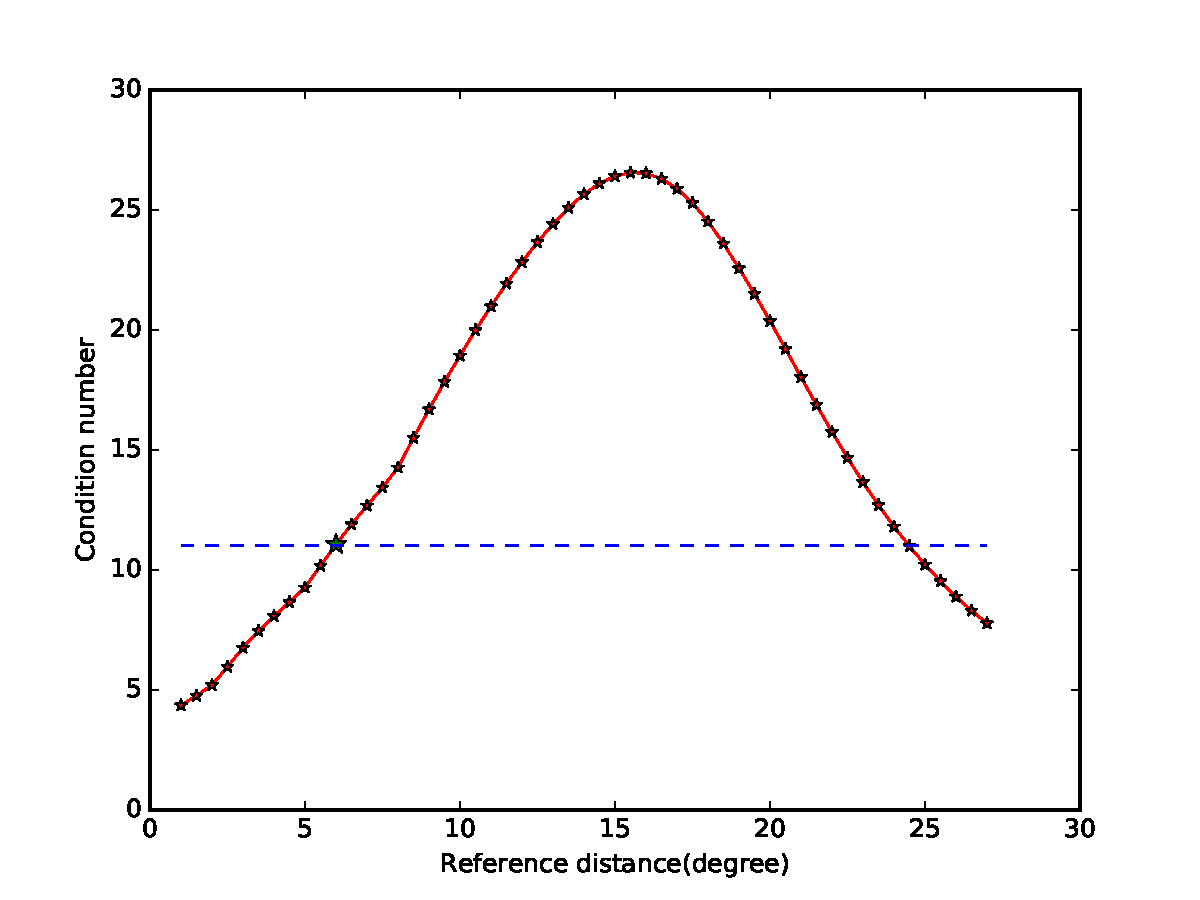
\includegraphics[width=.95\textwidth]{ch-weighting/figures/source_weight_cond_num.pdf}
  \caption[Condition number curve of the diagonal weighting matrix]
  {\small{Condition number of the diagonal weighting matrix defined by eqn.~(\ref{eq:spatial_weights})
as a function of the reference distance~$\Delta_0$\,.
The chosen value, indicated by the green star, is about one third of the largest possible value.
Since evaluation of eqn.~(\ref{eq:spatial_weights}) for different reference distances adds negligible computational expense, it is possible (and recommended) to repeat this type of analysis for each iteration.
}}
\label{fig:weight_condnum}
\end{figure}

Based on this choice, Figures~\ref{fig:receiver_weights} and \ref{fig:source_weights} illustrate the
distribution of weights in a recent global adjoint tomography study~\cite{Lei2018}. In Figure~\ref{fig:receiver_weights},
USArray and European stations weights are brought down to about one-tenth of ocean island station weights. The source weighting is similar, with the contribution of individual Fiji Tonga events brought down to about one-tenth the contribution of intraplate events in Asia. This ratio between the minimum and maximum weights can be adjusted through the reference distance parameter, as informed by practical experience in a given inversion.

\begin{figure}
 \centering 
   	\begin{minipage}[t]{.9\columnwidth}
  	\centering 
 	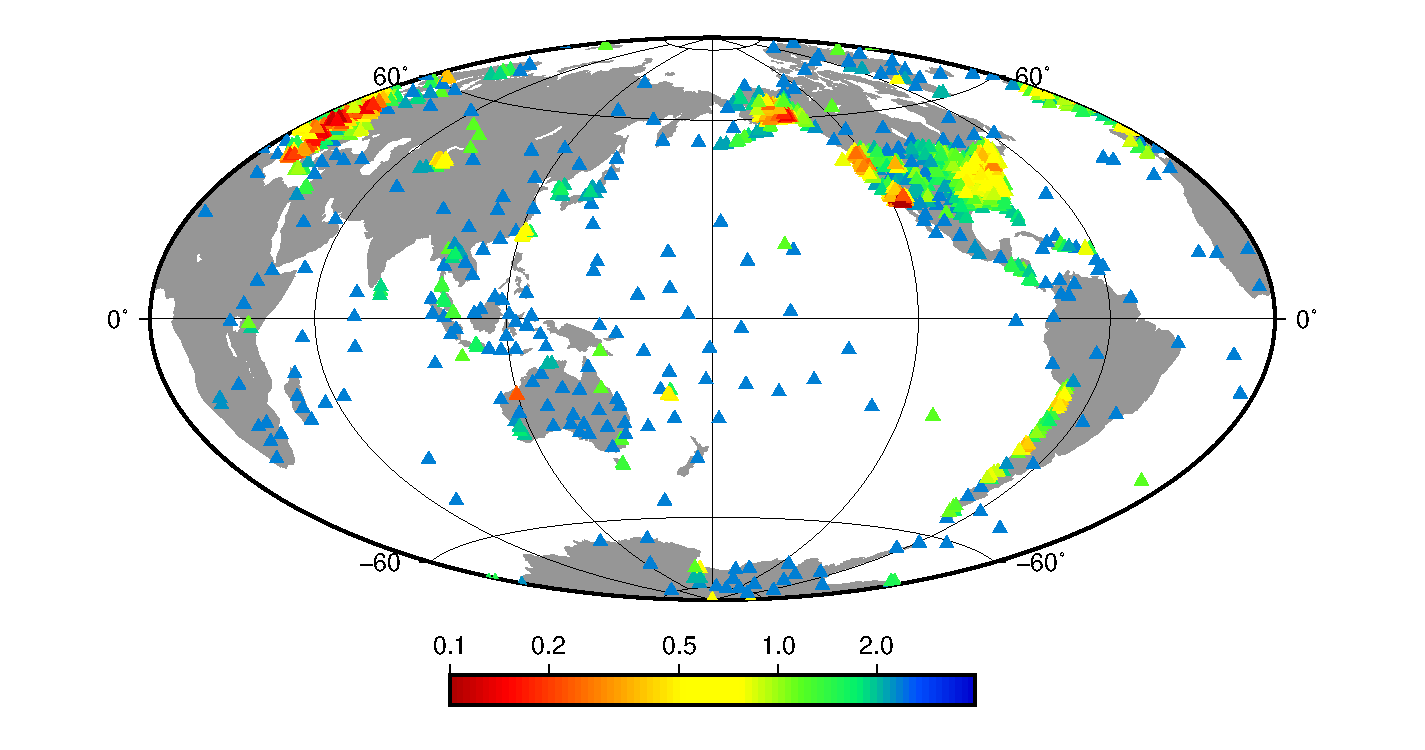
\includegraphics[width=.95\textwidth]{ch-weighting/figures/receiver-weights-40-100-Z.pdf}
	\end{minipage}
  \caption[Example of receiver weights]
  {\small{Example of receiver weights for an event C201604131355A at 40--100~s period band and vertical component determined based upon eqn.~(\ref{eq:spatial_weights}),
and normalized according to eqn.~(\ref{eq:recnorm}). The weights are in logarithmic scale.
Note the difference between USArray stations 
and ocean island stations. 
}}
\label{fig:receiver_weights}
\end{figure}

\begin{figure}
 \centering 
   	\begin{minipage}[t]{.9\columnwidth}
  	\centering 
	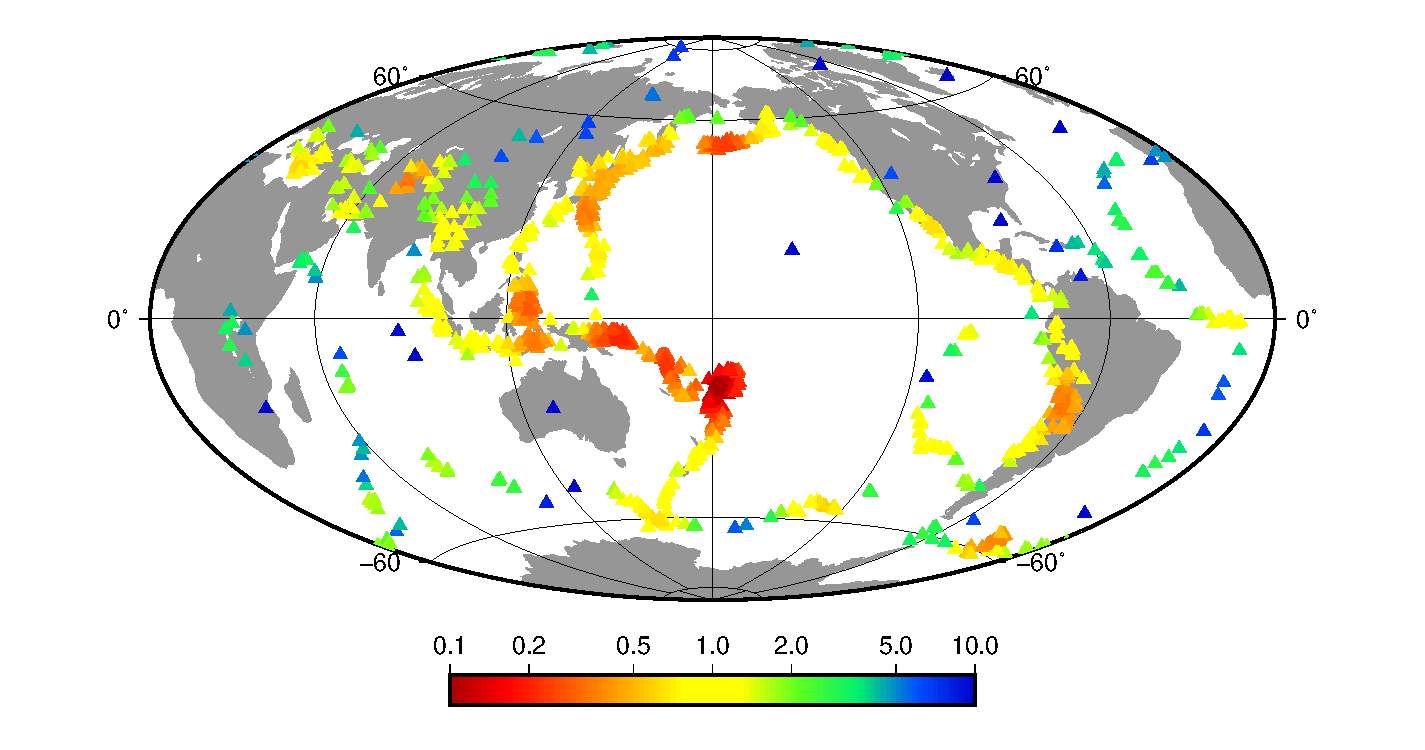
\includegraphics[width=.95\textwidth]{ch-weighting/figures/source-weights.pdf}
	\end{minipage}
  \caption[Example of source weights]
  {\small{Example of source weights determined based upon eqn.~(\ref{eq:spatial_weights}),
and normalized according to eqn.~(\ref{eqn:src_norm}).
Note the difference between dense subduction zone
earthquakes and sparse transform fault earthquakes.  
}}
\label{fig:source_weights}
\end{figure}

%===
\subsubsection{Weighting Normalization}
\label{sec:norm}

In this section our goal is to introduce geographical source and receiver weighting without changing the event- and category-level behavior of the misfit function discussed in Section~\ref{sec:simple}.  

In geometrical ray-based tomography, specific phases are identified and windowed. These phases usually correspond to distinct paths that provide constraints 
on different parts of Earth's interior, and some phases may be assigned more weight than others 
depending on the aims of the researcher.
In waveform inversion, any part of the wave train can 
be selected and phase identification is no longer required. We thus assign a uniform weight to all windows in a  seismogram,
\begin{equation}
\label{eq:I_omega_scrw}
\omega_{scrw} = 1
\quad ,
\end{equation}
such that, according to eqn.~(\ref{eq:simple_scr}), $\chi_{scr}\sim N_{scr}$.
The normalization of the geographical source weights from eqn.~(\ref{eq:spatial_weights}) 
is then determined in a straightforward manner by
\begin{align}
\label{eqn:src_norm}
\sum_{s=1}^{S} \omega_{s} = S
\quad .
\end{align}

Because the number of receivers that happen to be online varies from one source to another, including receiver weights in an inversion is not as straightforward.
To guide the normalization of receiver weights, we adopt the same type of analysis performed in connection with category-weighting and eqn.~(\ref{eq:catlev}).

If the model fits the data to 
within one standard deviation, the misfit in a certain source and category ~$\chi_{sc}$ approaches~$N_{sc}$, and the receiver-level misfit ~$\chi_{scr}$ approaches~$N_{scr}$ 
(eqns.~\ref{eq:simple_scr}--\ref{eq:simple_cs}).
These properties of the misfit imply a normalization requirement for the receiver weights~$\omega_{scr}$, 
determined by eqn.~(\ref{eq:spatial_weights}) for a given category~$c$ and source~$s$:
\begin{align}
\label{eq:recnorm}
\sum_{r=1}^{R_{sc}} \omega_{scr} \, N_{scr} = N_{sc}
\quad .
\end{align}
When~$\omega_{scr} = 1$, as in the simple weighting strategy, this normalization 
condition is naturally satisfied because
\begin{equation}
\sum_{r=1}^{R_{sc}} N_{scr} = N_{sc}
\quad .
\end{equation}
After we determine the source and receiver weights, what is left is to examine the category weights~$\omega_c$\,.
For the misfit function given by eqn.~(\ref{eq:misfit}), we want the contributions from each category to be balanced, 
and this implies that
\begin{align}
\omega_{c} \sum_{s=1}^{S}\, \omega_s \sum_{r=1}^{R_{sc}} \omega_{scr}\,N_{scr}
=
\omega_{c} \sum_{s=1}^{S} \omega_s\, N_{sc}
= \frac{1}{C} 
\quad ,
\end{align}
and thus
\begin{align}
\omega_{c} = \frac{1}{C}\,\frac{1}{ \sum_{s=1}^{S} \omega_s\, N_{sc}}
\quad .
\end{align}
Note that when~$\omega_s=1$, the weighting reduce to the category-weighting strategy, namely
\begin{align}
\omega_{c} = \frac{1}{C}\,\frac{1}{ N_{c}}
\quad .
\end{align}

From the normalization of geographical weights described above, we see that when the model 
fits the data to within one standard deviation, the source-level misfit ~$\chi_{sc}$ approaches~$N_{sc}$
and category-level misfit~$\chi_{c}$ approaches~$N_{c}$.

In theory, data correlation changes the degrees of freedom in the data space 
of an inversion.
Loosely speaking,
the above normalization can be thought of as changing  the degrees of freedom of the dataset for a given category~$c$ and source~$s$, as well as the degrees of freedom of the dataset in a given category~$c$.
Geographical weighting can be viewed as an approximation of the complete 
data covariance matrix. 
%%%%%------------------------------------------
%
%   2, 
%
%%%%---------------------------------------------
\section{Numerical Validation: 2D Global Adjoint Tomography}

\begin{figure}
    \centering
    \begin{minipage}[t]{.9\columnwidth}
    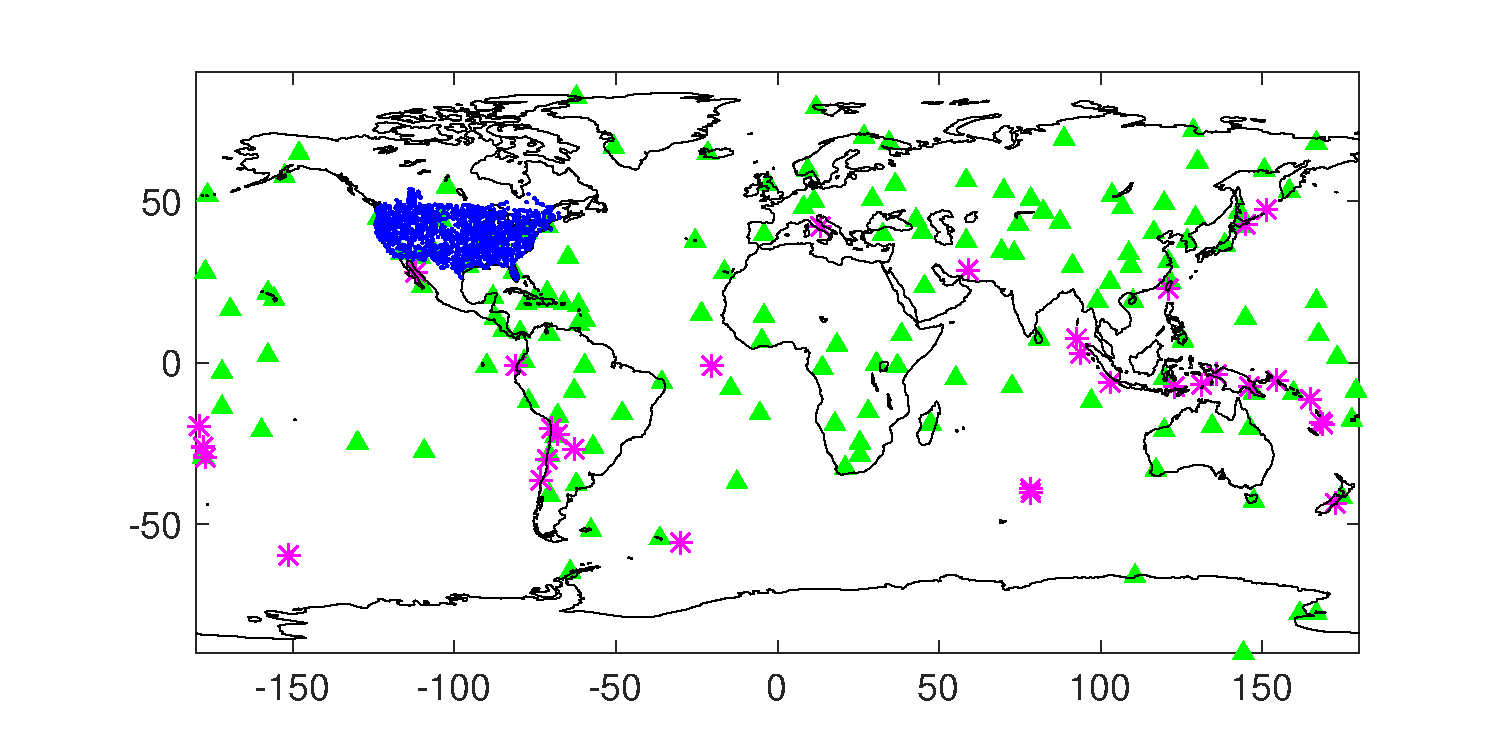
\includegraphics[width=.95\textwidth]{ch-weighting/figures/network.pdf}  %\\
    \end{minipage}
  \caption[source-receiver geometry used in synthetic inversions]
  {\small{Source-receiver geometry used in synthetic inversions.  
GSN stations are labeled by green triangles, USArray stations by blue trangles, and sources 
by magenta asterisks.
}}
\label{fig:test-src-sta}
\end{figure}

To test the geographical weighting strategy, 
we performed 2D inversions with a global test problem.  In these experiments, we used both GSN stations, which are sparsely distributed 
at the global scale, and USArray stations, which densely cover the North American continent, as shown in Figure~\ref{fig:test-src-sta}.
For the target model, we employed the acoustic test case  shown in Figure~\ref{fig:test-model}.  We generated synthetic data for this model using periodic boundary 
conditions at the edges to approximate a spherical Earth.  Finally, we inverted these data  with the workflow described by~\cite{Modrak2018}.  

\begin{figure}
    \centering
    \begin{minipage}[t]{.9\columnwidth}
    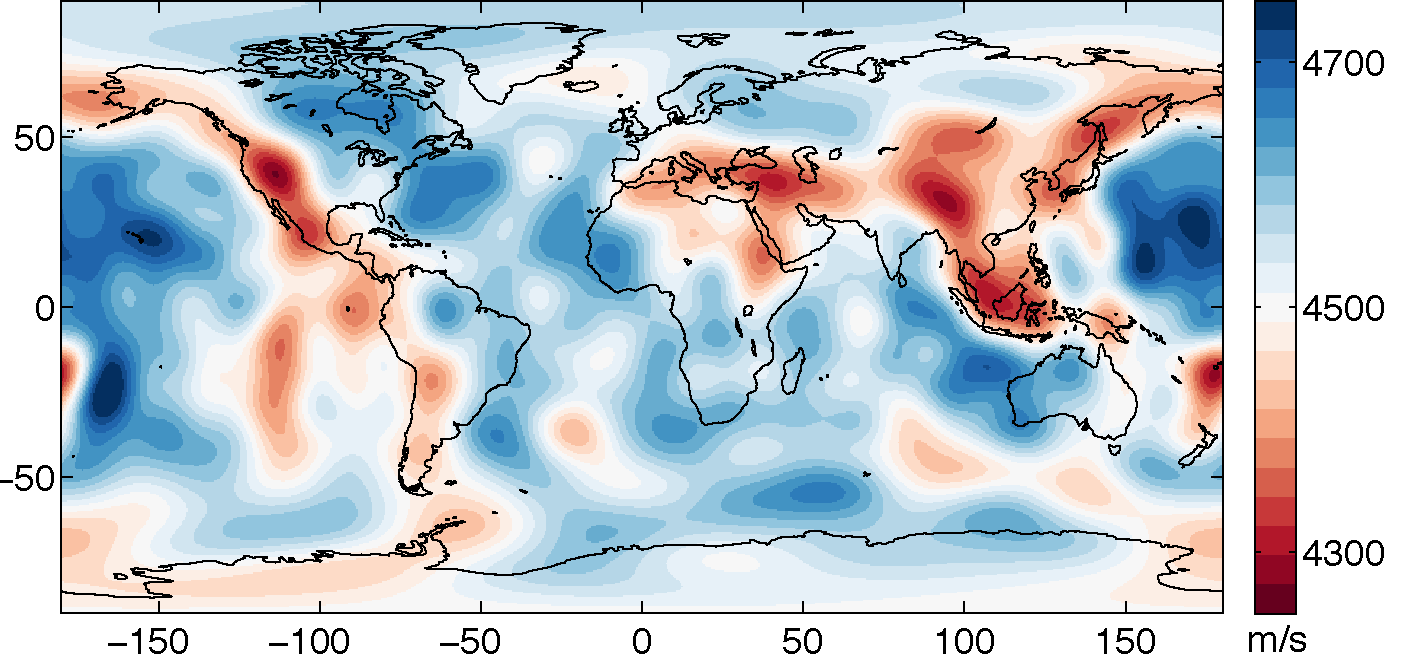
\includegraphics[width=.9\textwidth]{ch-weighting/figures/2Dmodel.pdf}  %\\
    \end{minipage}
  \caption[Target model used in the synthetic inversions for testing weighting strategies]{\small{Target model used in the synthetic inversions. Wavespeeds are determined by the 40~s Rayleigh wave phase speed model of~\cite{Trampert2003}.
}}
\label{fig:test-model}
\end{figure}
 
Starting from a homogeneous model, we tracked the reduction in model error as a function of the number of wavefield simulations in three separate inversions.
In the first inversion, we employed model-space diagonal preconditioning, using the best-performing preconditioner of all the variants tested by~\cite{Modrak2016}.
In the second inversion, we employed the category-weighting 
strategy discussed in Section~(\ref{sec:simple}).  
 In the third inversion, we used the geographical-weighting strategy described in Section~\ref{sec:geographical_weights}. The performance of the three methods is shown in Figure~\ref{fig:convergence}. 

\begin{figure}
    \centering
    \begin{minipage}[t]{.9\columnwidth}
    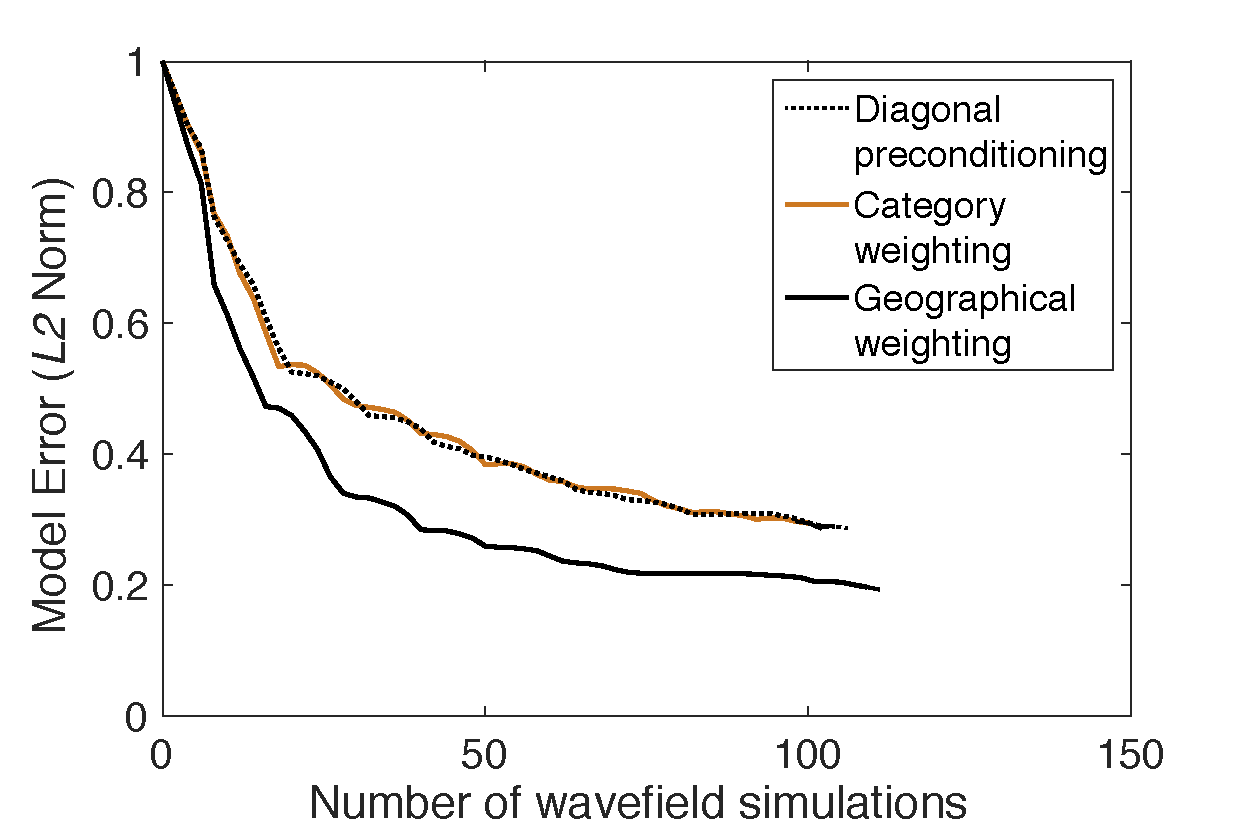
\includegraphics[width=.8\textwidth]{ch-weighting/figures/convergence_tests.pdf}  %\\
    \end{minipage}
  \caption[Convergence Test for different weighting strategies]
  {\small{With the category weighting defined in Section~\ref{sec:simple}, convergence is extremely slow.  
With the geographical weighting discussed in Section~\ref{sec:geographical_weights}, convergence is much faster.  
Diagonal model-space preconditioning, it turns out, is not an effective alternative to weighting when dealing with extremely lopsided source-receivers distributions.
}}
\label{fig:convergence}
\end{figure}

Compared with category weighting, preconditioning fails to provide an effective improvement, while the geographical-weighting 
strategy provides a much faster convergence rate. Considering the high cost of large-scale inverse problems 
like global adjoint tomography, where one iteration can require  millions of core hours, 
the saving could be significant. In addition to the performance improvement, the geographically-weighted inversion 
 demonstrates larger model error reduction than the other  approaches. 
%%%%%------------------------------------------
%
%   3, 
%
%%%%-------------------------------------------
\section{Application to 3D Global Adjoint Tomography: Misfit Statistics}

\begin{figure}
\centering
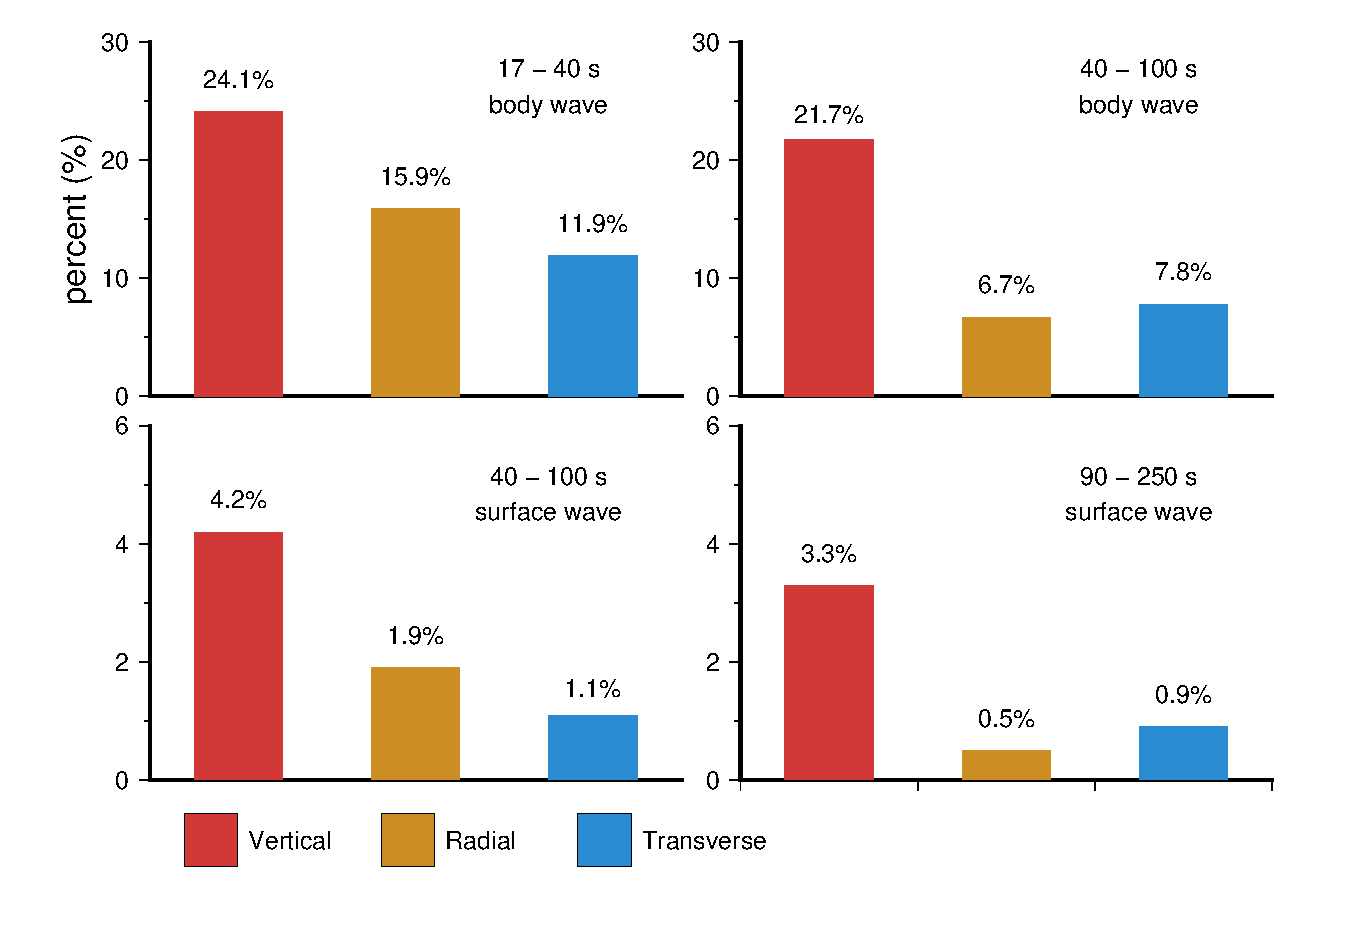
\includegraphics[width=0.8\textwidth]{ch-weighting/figures/category_wincount_contribution.pdf}
  \caption[Percentage of data in the twelve categories]
  {\small{Percentage of data (window count) in each of the twelve categories (see Table~\ref{table:categories}).
Period band and wave type are  labeled in the upper right corner of each panel.
Note the dramatic differences between  
body-wave (top) and surface-wave data (bottom). 
The large variations in data count from category to category illustrate the 
need for balancing.
}}
\label{fig:wcounts_contribution}
\end{figure}

After testing the geographical-weighting strategy through synthetic experiments,
we deployed it in our ongoing
global adjoint tomography study~\cite{Lei2018} with the goal of obtaining faster convergence and a 
better model. In this section we illustrate various aspects of the above category- and geographical-weighting
strategies.. 

\begin{figure}
\centering
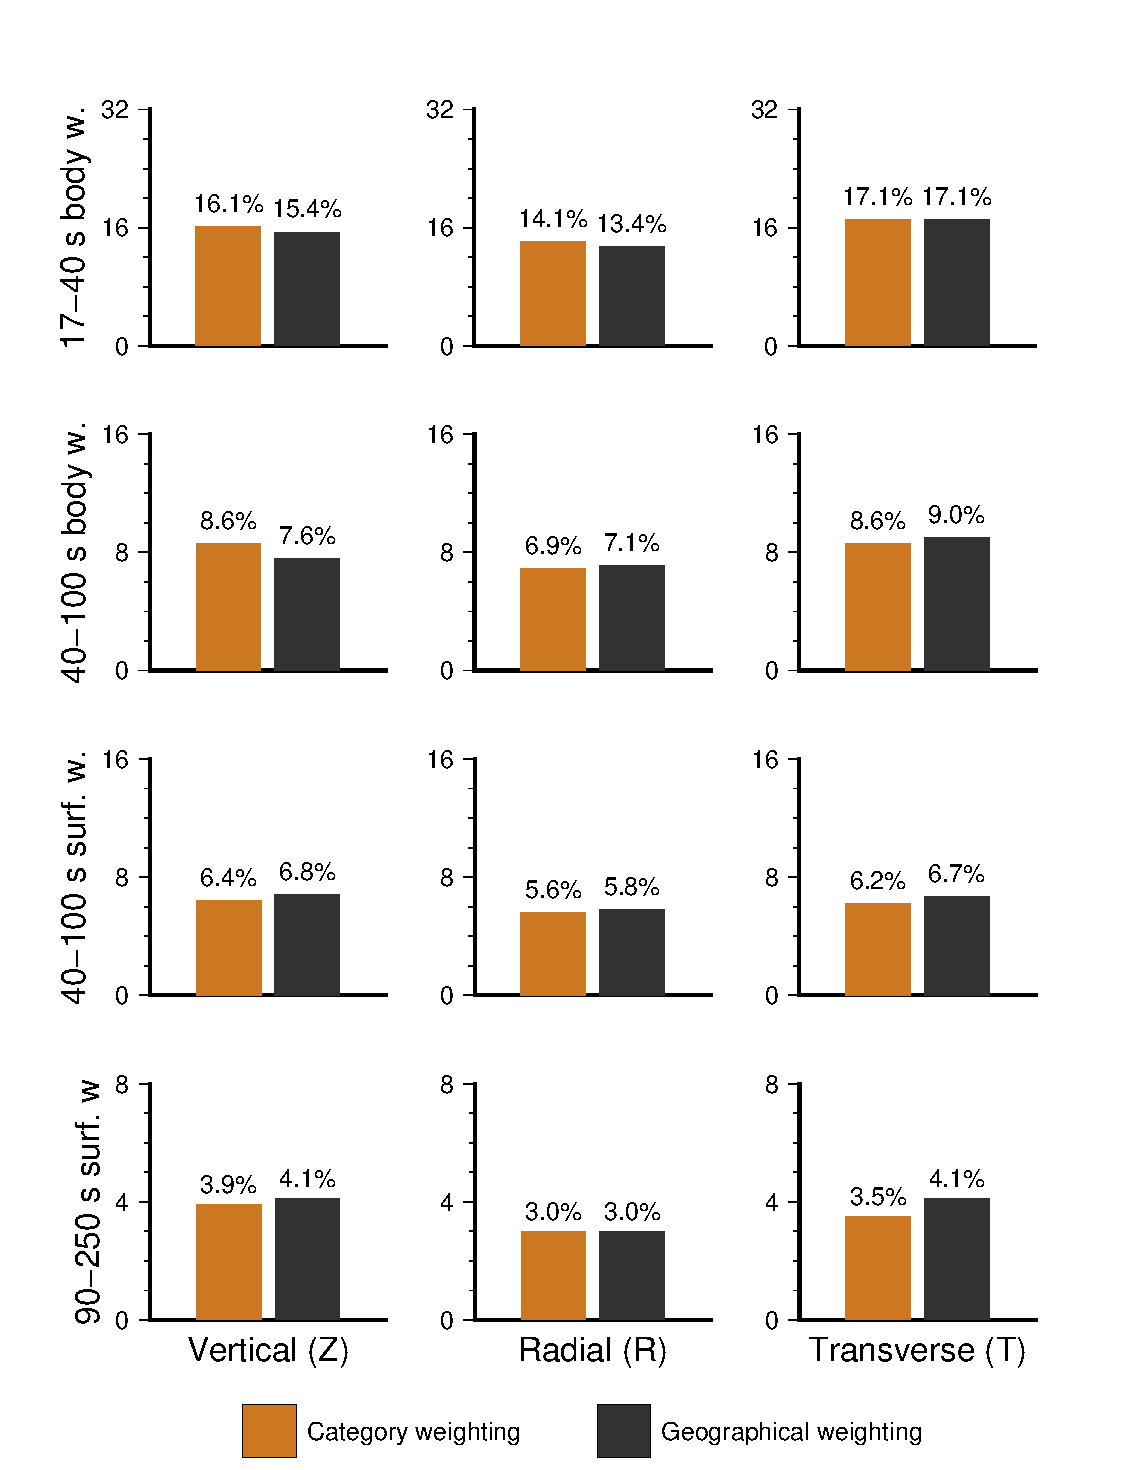
\includegraphics[width=0.8\textwidth]{ch-weighting/figures/category_misfit_contribution_color.pdf} 
  \caption[Percentage of the misfit in twelve categories]
  {\small{Percentage of the misfit in each of the twelve categories (see Table~\ref{table:categories}) using the category-weighting strategy (orange),
and geographical-weighting 
strategy (black). The percentage contribution in each category is labeled above the bars. Note that each category's contribution to the misfit barely changes with geographical weighting, because weight re-balancing only happens within each category.
}}
\label{fig:weights_histogram}
\end{figure}

As described in Section~\ref{sec:dataproc}, the weight we assign to each measurement is the product of source, category, receiver, 
and window weights: $\omega_{s}\, \omega_{c} \,\omega_{scr}\, \omega_{scrw}$\,.
In Figures~\ref{fig:receiver_weights}~and~\ref{fig:source_weights},
we plotted weights~$\omega_{s}$ assigned to sources and weights~$\omega_{scr}$ assigned to receivers.  
Next, we examine the misfit when the product of all four weights is applied.  

In total, we picked more than 17 million windows from 1,480 sources and 12 categories~\cite{Lei2018}. 
As shown in Figure~\ref{fig:wcounts_contribution}, 
the contribution from each category is far from balanced.  Short period body-wave data (17--40 s)
account for more than 50\% of the total number of windows while long period surface waves (90--250 s) contribute less than 5\%.
Across all three periods bands, more than 80\% of windows correspond to body-wave data.  For a given period band, the vertical component always provides more 
data than the horizontals.
If not balanced, these differences between categories can cause regions 
sensitive to body waves to be updated more than regions sensitive to surface waves and slow down the overall convergence rate.    

We define the weighted misfit for each category as
\begin{equation}
\Phi_{c} = \sum_{s=1}^{S} \sum_{r=1}^{R_{sc}} \sum_{w=1}^{N_{scr}} \omega_s\, \omega_{c} \,\omega_{scr}\, \omega_{scrw}\, \chi_{scr}
\end{equation}
In Fig.~\ref{fig:weights_histogram}, we calculate the percentage of the summed misfit for each category 
using two weighting strategies: (1) Orange bars correspond to category-only weighting, and (2) black bars correspond to the full category- and geographical-weighting strategy.

\begin{figure}
\centering
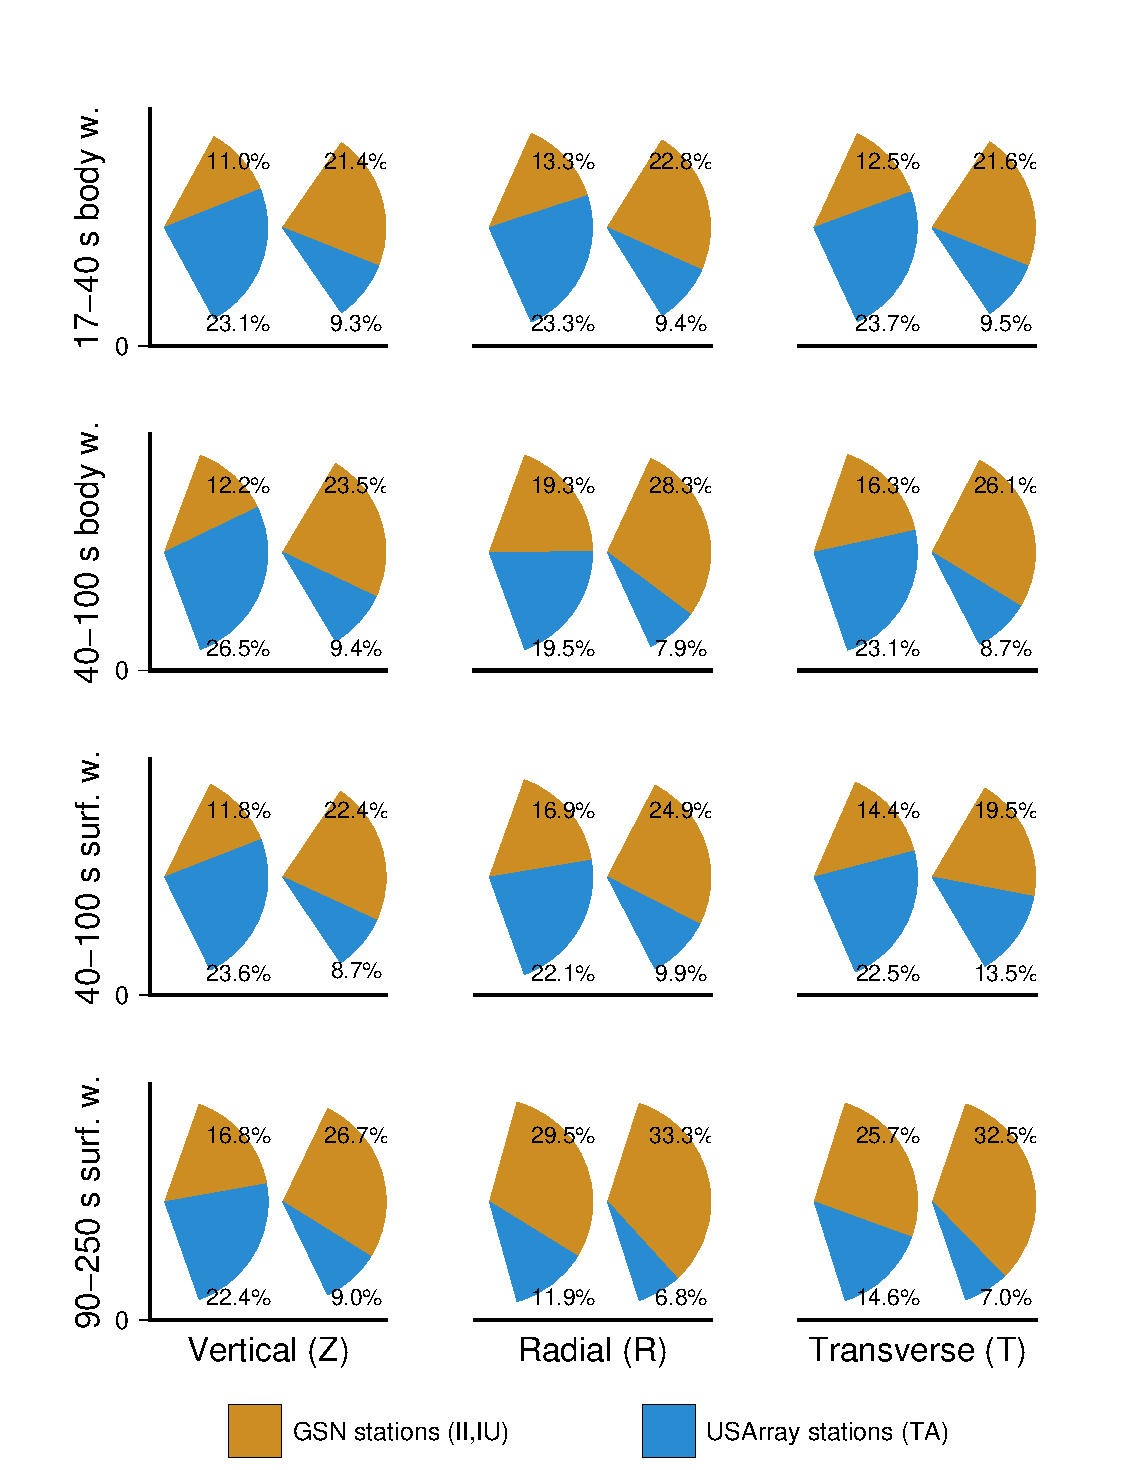
\includegraphics[width=0.85\textwidth]{ch-weighting/figures/category_sta_misfit_contribution.pdf}
  \caption[Percentage of the misfit of GSN stations and USArray stations]
  {\small{Percentage of the misfit of GSN stations (II, IU) and USArray stations (TA)
in each category using category-weighting (left wedges in each panel) and geographical-weighting
strategies (right wedges in panel).
Compared with the category-weighting strategy, the geographical-weighting 
strategy assigns more weight to GSN stations and down weights USArray stations in all categories.
}}
\label{fig:weights_contribution_sta}
\end{figure}

In the first case, after employing the category-weighting strategy in which the misfit is normalized by the 
total number of data in each category (Fig.~\ref{fig:wcounts_contribution}), misfits from different categories are better balanced 
and do not vary dramatically from category to category.  Although the 
summed weights themselves are equal in each category, the weighted misfits from each category 
are not.  The weighted misfits of short-period body waves are on average 2 to 3 
times larger than the misfits of long-period body and surface waves. We attribute this to the larger number of updates required to fit short-period phases compared with long-period phases, and we expect the body-wave misfits to decrease as the inversion progresses. 

In the second case, when geographical weighting is applied, the distribution of 
misfits in each category does not significantly change, meaning that the  re-balancing happens only within each category, as desired.

To further probe the overall re-balancing within each category, we compare the contribution to the total misfit from  two seismographic networks:  USArray (network ID TA) and GSN (network IDs II and IU).
USArray stations are densely distributed across North America and GSN stations are sparsely distributed across the  globe.

The total  misfit from USArray or GSN stations in each category is given by
\begin{equation}
\Phi_{c}^{\text{\scriptsize USArray / GSN}} = \sum_{s=1}^{S} \sum_{r=1}^{R_{sc}} \sum_{w=1}^{N_{scr}} \omega_s\, \omega_{c}\, \omega_{scr}\, \omega_{scrw}\,\chi_{scr}^{\text{\scriptsize USArray / GSN}}
\end{equation}
Fig.~\ref{fig:weights_contribution_sta} shows the percentage of~$\Phi_{c}^\text{\scriptsize USArray}$ and  
$\Phi_{c}^\text{\scriptsize GSN}$ in each category under different weighting strategies.
In the category-weighing strategy, GSN stations contribute much less to the overall misfit than  
USArray stations, reflecting the proportionality to the amount of data, as expected.
In the geographical-weighting strategy, the contribution 
of GSN stations is enhanced due to the re-balancing. 

\begin{figure}
\centering
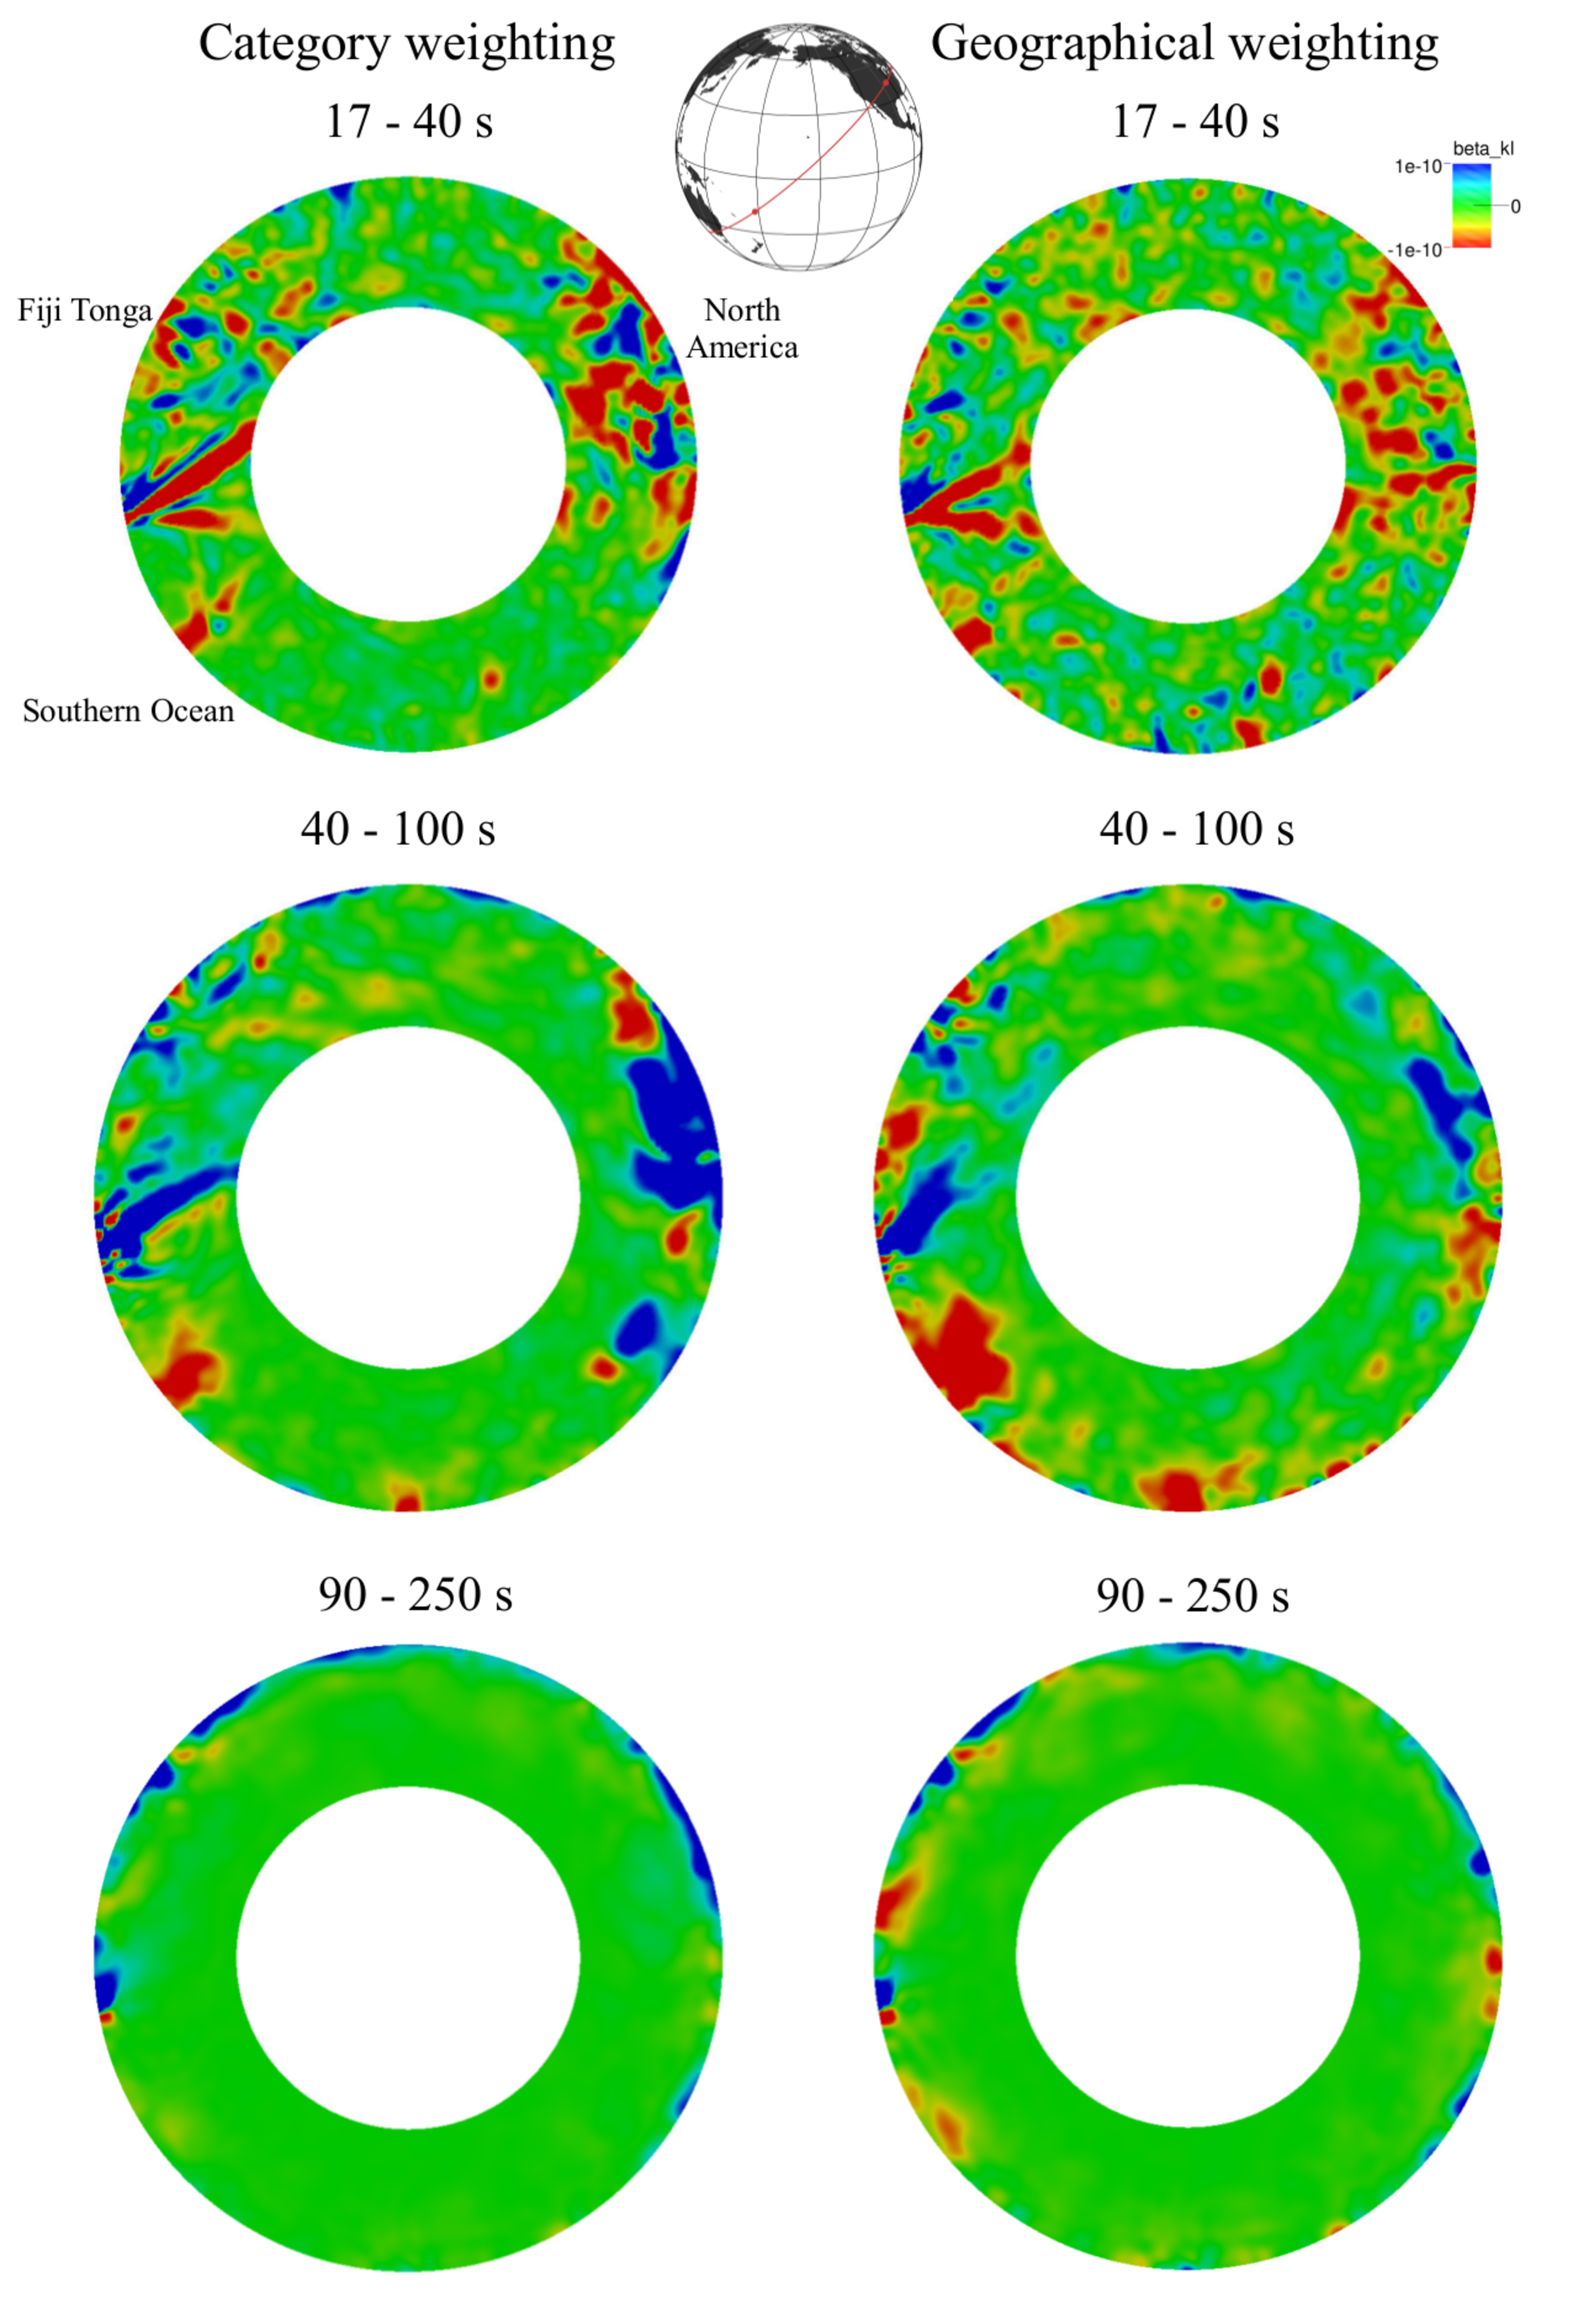
\includegraphics[width=0.85\textwidth]{ch-weighting/figures/Figure-10-small.pdf}
  \caption[Smoothed gradient contributions w/ and w/o weightings applied]
  {\small{Smoothed gradient contributions using data from 42 earthquakes without (Left Column) 
and with source \& receiver weighting (Right Column) in three
period bands: 17--40~s (Top Row), 40--100~s (Middle Row), and 90--250~s (Bottom Row). The top center map shows the cross section with red line for reference.   
The isotropic smoothing length scale is 100~km.
}}
\label{fig:gradient_category}
\end{figure}

To further illustrate the effects of weighting, we selected 42 events for a 
pilot test and examined the model update gradient. Ideally, we should run forward and adjoint simulations for 
each of the 12 categories for one weighting strategy, and repeat this process for the other weighting strategy, which would require 2,016
simulations in total.
To save computational cost while keeping the test meaningful,
we considered only three categories, 17--40~s, 40--100~s, 
and 90--250~s, and ignored wave types for the adjoint simulations. 
Fig.~\ref{fig:gradient_category} shows cross sections of the model update gradient.
In the shortest period band (17--40~s),
the gradient based on category-weighting is
dominated by regions beneath Fiji Tonga and North America,
with limited updates in the southern hemisphere.
In contrast, the geographical-weighting approach results in a balanced gradient with
more information in the southern hemisphere and relatively reduced sensitivity beneath Fiji Tonga and North America.  
The longer period bands, involving mostly surface waves,
demonstrate similar behavior but more focused on the shallow mantle.  
Upon combining all three categories, we clearly see that the model update based on the geographical 
weighting strategy is better balanced, with a more even sampling of the whole mantle (Fig.~\ref{fig:gradient_sum}).  
From this pilot test we conclude that the geographical-weighting strategy effectively 
balances the inversion and improves the convergence rate, which is necessary for any inversion dealing 
with the unevenly distributed data.

\begin{figure}
\centering
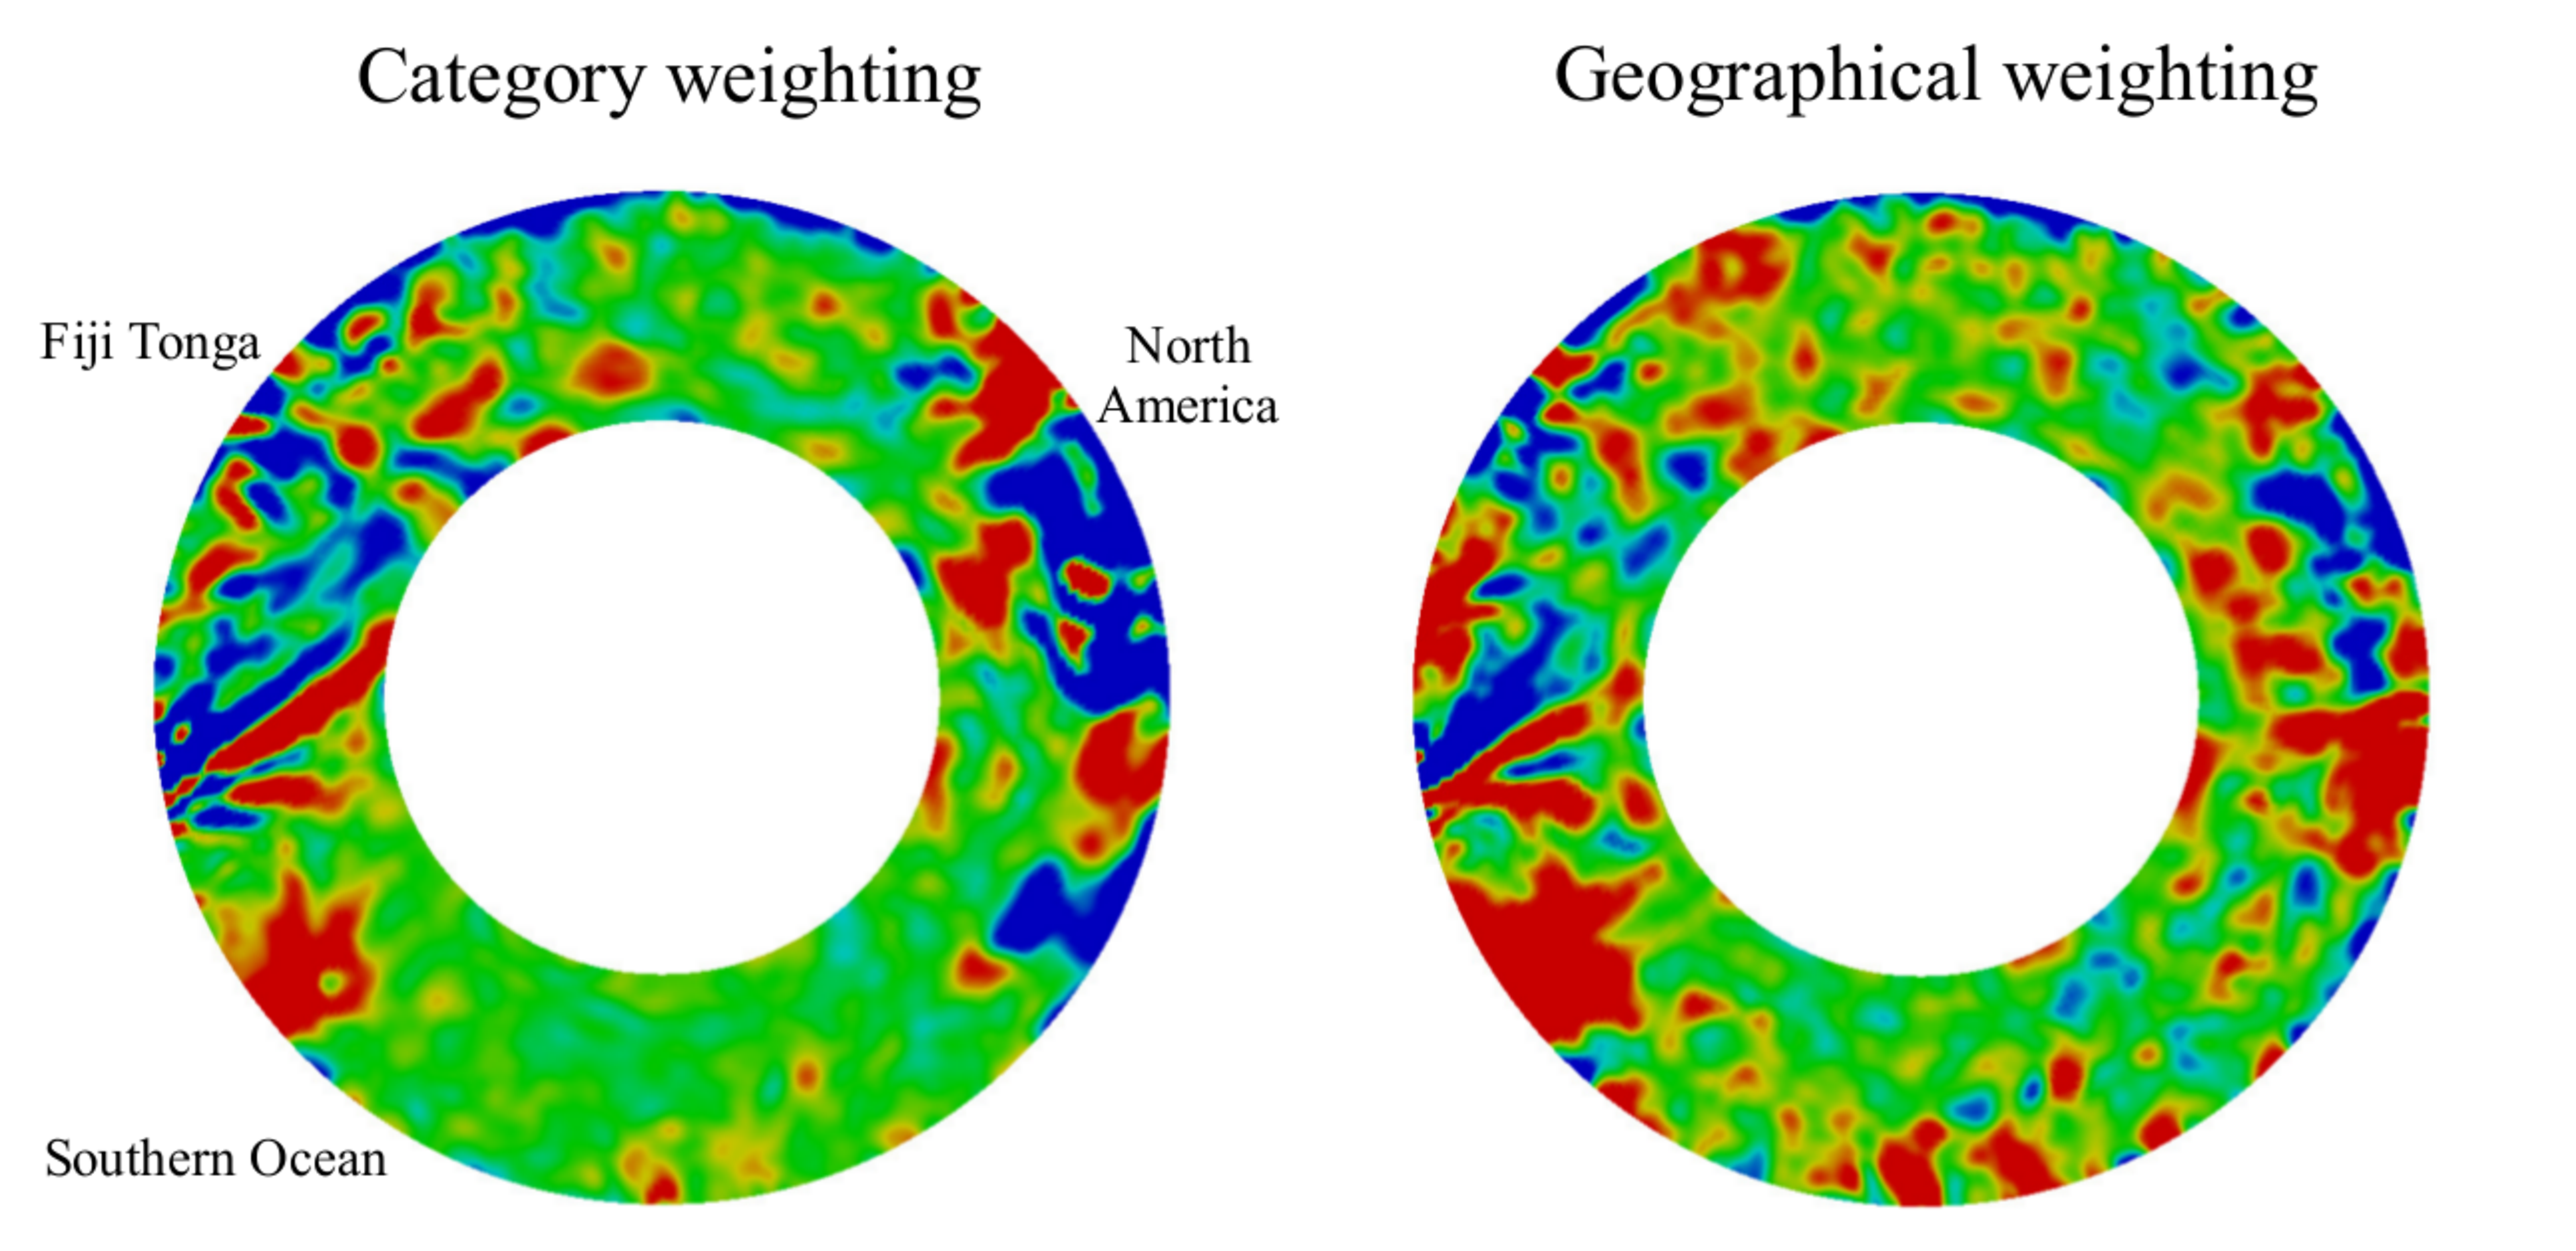
\includegraphics[width=0.85\textwidth]{ch-weighting/figures/Figure-11-small.pdf}
  \caption[Example of the summation of smoothed misfit gradients from three period bands]
  {\small{Example of a smoothed misfit gradient (weighted summation of the contributions of the three period bands shown in Fig.~\ref{fig:gradient_category}) 
using data from 42 earthquakes without (Left) and with source \& receiver weighting (Right). The isotropic smoothing length scale is 100~km.
}}
\label{fig:gradient_sum}
\end{figure}

% \subsection{Weighting double-difference Measurements}
% The geographical-weighting strategy introduced above can be adapted to other scenarious with uneven 
% data coverage. For instance, in the double difference inversion~\citep[e.g.,][]{Yuan2016} where the difference between 
% station are used as the misfit, a dense regional array will have many more station pairs than individual stations, 
% the inversion can suffer from even greater lopsidedness than conventional ones.  The station weights introduced in Section~\ref{sec:geographical_weights} (Top in Fig.~\ref{fig:dd_weights} for reference) can be adapted 
% to double difference case.  To address the unevenness of data coverage in double-difference inversion,
% we introduce an additional term~$P_{csi}$, the number of the station pairs associated with a single station, to balance the 
% contribution of station pairs. The geographical distribution of not individual stations but rather of stations pairs then 
% leads to a modified receiver weighting,
% \begin{equation}
% 	\omega_{csr} = \left( \sum_{i=1}^{R_{cs}} P_{csi} \exp\left[\mbox{}-\left(\frac{\Delta_{ir}}{\Delta_{0}}\right)^2\right] \right)^{-2} \quad ,
% \label{eq:dd_weights}
% \end{equation}
% where~$P_{csi}$ is the number of station pairs associated with the~$c$-th category,~$s$-th source, and~$i$-th receiver.  
% The normalizations and category weights described in Section~\ref{sec:norm} 
% remain the same in the double difference case as in the conventional case. 
% We note that in the limit of~$\Delta_{0} \to 0$, eqn.~\ref{eq:dd_weights} simply reduces to~$\omega_{csr} = P_{csr}^{-2}$. 
% In Fig.~\ref{fig:dd_weights},  we show the effect of the additional term in the receiver weighting.  The bottom plot shows
% that the additional term~$P_{csi}$ combine with the geographical-weighting produces larger contrast between 
% the weights of dense receivers and sparse receivers and therefore better address the unevenness in double-difference data.  
% More detail of the implementation of this weighting strategy and it's effect on the double-difference tomography is beyond the 
% scope of this paper and will be discussed in ({\color{Red} reference of Orsvuran et al.})

%%%%%-------------------------
%
%  conclusions
%
%%%%%-------------------------
\section{Conclusion}

We propose a geographic weighting strategy to address uneven data coverage in seismic tomography.  %We demonstrated how we introduce the weighting strategy while preserving the degree of freedom of the data. 
To test the approach, we performed synthetic 2D global adjoint tomography experiments using realistic source and receiver distributions.  
The results show that geographical weighting performs better than category-only weighting and conventional diagonal model-space preconditioning. %More importantly, it not only avoids pathological behavior along array-events but also achieves the results much faster and converges closer to the target. 
%The results also approve that the geographical-weighting can be a good approximation of a complete data covariance matrix.  
A 42-event pilot test was used to illustrate how  
geographical weighting balances densely and sparsely sampled regions.  
Finally,
using a database of 1,480 earthquakes, we performed a statistical analysis of 17~million measurements assimilated in the global adjoint tomography inversion of~\cite{Lei2018}, verifying expected effects of the weighting scheme. 
As more data from dense regional seismographic networks become available, we expect weighting to play an increasingly important role in scientific studies of Earth's interior~\cite{Orsvuran2019}.    
